\chapter{周期流形}
\markboth{周期流形}{周期流形}

\begin{remark}[本章定位]\label{rem:periodic_manifold_chapter_positioning}
周期流形是周期数学中离散几何与离散分析的核心理论。本章从连续流形上的周期结构出发，建立\textbf{周期流形}的一般理论，再将其离散化为格点模型。本章的核心对象有三类：\textbf{周期流形}（带具有周期轨道的群的作用的流形）、\textbf{周期轨道}（闭曲线及其模空间）、\textbf{离散格点流形}（周期结构的离散化）。

本章的核心任务之一是\textbf{严格建立三大微分算子——梯度、散度、旋度——的完整理论}。在连续情形，我们给出它们的内蕴定义（不依赖坐标选择）和坐标公式；在离散情形，我们给出它们的严格推导（从泰勒展开和通量平衡出发）、精确恒等式（不需要取极限）和连续极限的完整证明。

\textbf{本章七主题导引}：平移——格点平移操作（定义 \ref{def:lattice_translation}）与离散梯度（定义 \ref{def:discrete_gradient_strict}）；缩放——格点缩放操作（定义 \ref{def:lattice_scaling}）与离散散度（定义 \ref{def:discrete_divergence_strict}）；旋转——格点旋转操作（定义 \ref{def:lattice_rotation}）与离散旋度（定义 \ref{def:discrete_curl_strict}）；守恒——离散幺正演化的模方守恒（命题 \ref{prop:unitary_norm_conservation}）、三大算子的积分定理（定理 \ref{thm:gauss_divergence_manifold}、\ref{thm:stokes_manifold}）；对称——离散性本原公理（公理 \ref{axm:discreteness}）与三个对称中心 $0,1,i$ 的对应；闭合——plaquette 的 Wilson 环闭合判据（引理 \ref{ch12_wilson_homotopy_lemma}）；周期——离散幺正算子的周期条件（命题 \ref{prop:discrete_period_condition}）。
\end{remark}

\begin{figure}[htbp]
\centering
\begin{tikzpicture}[
  font=\small,
  box/.style={draw, rounded corners, fill=blue!8, minimum width=2.6cm, minimum height=0.8cm, align=center},
  sub/.style={draw, rounded corners, fill=green!10, minimum width=2.4cm, minimum height=0.7cm, align=center, font=\footnotesize},
  arr/.style={->, thick, >=stealth}
]
  \node[box] (pm) {周期流形\\$M/G$};
  \node[box, right=1.0cm of pm] (po) {周期轨道\\$\pi_1(M)$};
  \node[box, right=1.0cm of po] (df) {微分形式\\de Rham 上同调};
  \node[box, right=1.0cm of df] (sp) {辛流形\\能量面};
  \node[sub, below=1.0cm of pm] (pb) {主丛与联络\\和乐};
  \node[sub, below=1.0cm of po] (it) {不变环面\\Liouville--Arnold};
  \node[sub, below=1.0cm of df] (mm) {模空间\\周期轨道族};
  \node[sub, below=1.0cm of sp] (dl) {离散格点\\本原公理};
  \node[box, fill=orange!12, below=1.0cm of $(pb)!0.5!(dl)$] (uni) {连续—离散统一：三大算子、幺正演化、Wilson 环};
  \draw[arr] (pm) -- (po);
  \draw[arr] (po) -- (df);
  \draw[arr] (df) -- (sp);
  \draw[arr] (pm) -- (pb);
  \draw[arr] (po) -- (it);
  \draw[arr] (df) -- (mm);
  \draw[arr] (sp) -- (dl);
  \draw[arr] (pb) -- (uni);
  \draw[arr] (it) -- (uni);
  \draw[arr] (mm) -- (uni);
  \draw[arr] (dl) -- (uni);
\end{tikzpicture}
\caption{本章结构总览：从周期流形出发，经周期轨道、微分形式、辛流形、主丛与联络，到不变环面、模空间与离散格点，最终统一于连续—离散对应。}
\label{fig:periodic_manifold_overview}
\end{figure}

\section{周期流形的基本结构}\label{sec:periodic_manifold_basic}

\begin{definition}[周期流形]\label{def:periodic_manifold}
设 $M$ 为 $n$ 维光滑流形，$G$ 为李群。称 $(M,G,\Phi)$ 为\textbf{周期流形}，若 $G$ 通过光滑左作用 $\Phi:G\times M\to M$ 作用于 $M$，且
\begin{enumerate}[label=(\roman*)]
    \item 作用自由：$g\cdot p=p\Rightarrow g=e$；
    \item 作用真不连续：对任意紧致 $K\subseteq M$，$\{g\in G:gK\cap K\neq\emptyset\}$ 为有限集；
    \item 轨道空间 $M/G$ 为光滑流形（商流形）。
\end{enumerate}
当 $G=\mathbb{Z}$ 或 $\mathbb{Z}^n$ 时，轨道为周期轨道；当 $G=U(1)$ 或 $\mathbb{T}^n$ 时，轨道为闭合轨道；当 $G=\mathbb{R}$ 时，轨道为流线。
\end{definition}

\begin{example}[环面作为周期流形]\label{ex:torus_periodic_manifold}
$n$ 维环面 $\mathbb{T}^n=\mathbb{R}^n/\mathbb{Z}^n$ 是周期流形的原型：$\mathbb{Z}^n$ 通过平移作用于 $\mathbb{R}^n$，作用自由且真不连续，商空间 $\mathbb{R}^n/\mathbb{Z}^n$ 微分同胚于 $S^1\times\cdots\times S^1$。
\end{example}

\begin{example}[透镜空间]\label{ex:lens_space}
设 $p,q$ 互素，$L(p,q)=S^3/\mathbb{Z}_p$，其中 $\mathbb{Z}_p$ 通过 $(z_1,z_2)\mapsto(e^{2\pi i/p}z_1,e^{2\pi i q/p}z_2)$ 作用于 $S^3\subseteq\mathbb{C}^2$。$L(p,q)$ 是周期流形，其基本群为 $\mathbb{Z}_p$，所有闭轨道均为有限阶扭绕轨道。
\end{example}

\begin{figure}[htbp]
\centering
\begin{tikzpicture}[scale=0.9]
  % 左：万有覆叠 R
  \draw[->, thick, >=stealth] (-3.5,0) -- (3.5,0);
  \foreach \x in {-3,-2,-1,0,1,2,3} {
    \node[circle, fill, inner sep=1pt] at (\x,0) {};
  }
  \node at (0,-0.5) {$\mathbb{R}$};
  \foreach \x in {-3,-2,-1,0,1,2,3} {
    \node[below, font=\footnotesize] at (\x,-0.1) {\x};
  }
  % 右：商流形 S^1
  \draw[->, thick, >=stealth, red] (-2,0.2) .. controls (-2,1.5) and (2,1.5) .. (2,0.2);
  \node[red] at (0,1.7) {$\pi(t)=e^{2\pi it}$};
  \draw[thick, fill=orange!10] (0,-3.5) circle (1.0);
  \node[circle, fill, inner sep=1.5pt] at (1.0,-3.5) {};
  \node at (1.4,-3.5) {$1$};
  \node at (0,-4.8) {$S^1$};
  \node at (0,-2.4) {万有覆叠};
\end{tikzpicture}
\caption{实直线 $\mathbb{R}$ 是圆周 $S^1$ 的万有覆叠：$\pi(t)=e^{2\pi i t}$，纤维为 $\mathbb{Z}$。}
\label{fig:covering_R_S1_periodic}
\end{figure}

\begin{proposition}[商流形的光滑性]\label{prop:quotient_smooth}
设 $G$ 为紧致李群，自由光滑作用于流形 $M$。则轨道空间 $M/G$ 具有唯一光滑结构使投影 $\pi:M\to M/G$ 为光滑浸没。
\end{proposition}

\begin{proof}
由自由作用，每条轨道为嵌入子流形且与 $G$ 微分同胚。对任意 $p\in M$，存在 $G$-不变邻域 $U$ 与切片 $S$ 使 $U\cong S\times G$，其中 $S$ 横截轨道。$M/G$ 的局部坐标由 $S$ 给出，转移函数的光滑性由 $G$-作用的自由性保证。唯一性由商拓扑的泛性质给出。参见 \cite{wang2023manifolds}。
\end{proof}

\begin{remark}[与“流形基础与纤维丛”章的关系]\label{rem:periodic_manifold_relation}
本章的周期流形理论直接建立在“流形基础与纤维丛”章建立的连续流形理论之上。环面作为商流形（命题 \ref{prop:torus_quotient}）、覆叠空间（定义 \ref{def:covering_space}）、基本群（定义 \ref{def:closed_orbit_manifold}）、不变环面（定义 \ref{def:invariant_torus}）、辛结构（定义 \ref{def:phase_space_cotangent}）等概念在本章中被系统使用，而非重新发明。
\end{remark}

\section{周期轨道与基本群}\label{sec:periodic_orbit_fundamental_group}

\begin{definition}[闭合轨道与扭绕]\label{def:closed_orbit_twisting}
设 $\gamma:[0,T]\to M$ 为闭合轨道。$\gamma$ 定义基本群中的元素 $[\gamma]\in\pi_1(M)$。若 $[\gamma]$ 为有限阶元素（阶为 $p$），则称 $\gamma$ 为\textbf{$p$ 阶扭绕闭合轨道}。
\end{definition}

\begin{remark}[环面基本群的来源]\label{rem:torus_fundamental_group_source}
\cref{prop:periodic_manifold_fundamental_group} 已在「流形基础与纤维丛」章证明并给出（含证明）；本节直接引用，不重复陈述。
\end{remark}

\begin{corollary}[扭绕轨道的判定]\label{cor:twisted_orbit}
设 $\gamma$ 为 $\mathbb{T}^n$ 上的闭合轨道，$[\gamma]=(k_1,\dots,k_n)\in\mathbb{Z}^n$。则 $\gamma$ 为有限阶扭绕轨道当且仅当 $(k_1,\dots,k_n)$ 为 $\mathbb{Z}^n$ 中的有限阶元素，即 $(k_1,\dots,k_n)=(0,\dots,0)$。
\end{corollary}

\begin{proof}
$\mathbb{Z}^n$ 是无挠阿贝尔群，除零元外无有限阶元素。故仅平凡元素对应有限阶扭绕轨道。
\end{proof}

\begin{figure}[htbp]
\centering
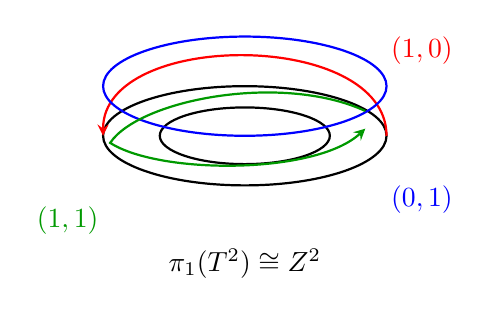
\begin{tikzpicture}[scale=0.9]
  % 环面
  \draw[thick] (0,0) ellipse (2.0 and 0.7);
  \draw[thick] (0,0) ellipse (1.2 and 0.4);
  % 经线闭环 (1,0)
  \draw[thick, red, ->, >=stealth] (2.0,0) .. controls (2.0,1.5) and (-2.0,1.5) .. (-2.0,0);
  \node[red] at (2.5,1.2) {$(1,0)$};
  % 纬线闭环 (0,1)
  \draw[thick, blue, ->, >=stealth] (0,0.7) ellipse (2.0 and 0.7);
  \node[blue] at (2.5,-0.9) {$(0,1)$};
  % 对角闭环 (1,1)
  \draw[thick, green!60!black, ->, >=stealth] (1.7,0.35) .. controls (0.5,0.9) and (-1.5,0.5) .. (-1.9,-0.1)
                                          .. controls (-1.2,-0.55) and (1.0,-0.55) .. (1.7,0.1);
  \node[green!60!black] at (-2.5,-1.2) {$(1,1)$};
  \node at (0,-1.8) {$\pi_1(\mathbb{T}^2)\cong\mathbb{Z}^2$};
\end{tikzpicture}
\caption{环面上的闭合轨道按 $\pi_1(\mathbb{T}^n)\cong\mathbb{Z}^n$ 中的整数向量分类。}
\label{fig:torus_fundamental_group_periodic}
\end{figure}

\section{周期流形上的微分形式}\label{sec:periodic_forms}

\begin{definition}[闭形式与恰当形式]\label{def:closed_exact_forms}
$k$-形式 $\omega$ 称为\textbf{闭形式}，若 $d\omega=0$。称为\textbf{恰当形式}，若存在 $(k-1)$-形式 $\eta$ 使 $\omega=d\eta$。恰当形式必为闭形式（$d^2=0$）。
\end{definition}

\begin{definition}[de Rham 上同调]\label{def:de_rham}
$M$ 的第 $k$ 个 \textbf{de Rham 上同调群}为
\[
H^k_{dR}(M):=\frac{\ker(d:\Omega^k(M)\to\Omega^{k+1}(M))}{\operatorname{im}(d:\Omega^{k-1}(M)\to\Omega^k(M))}.
\]
\end{definition}

\begin{theorem}[de Rham 定理]\label{thm:de_rham}
对光滑流形 $M$，$H^k_{dR}(M)\cong H^k(M;\mathbb{R})$（奇异上同调）。
\end{theorem}

\begin{proof}
\textbf{证明超出本书范围}。这是 de Rham 定理，其证明使用层论或谱序列方法。参见 \cite{lee2012smooth} 第 18 章。核心思想：de Rham 复形与奇异上链复形之间的双对偶给出自然同构。
\end{proof}

\begin{proposition}[周期积分与上同调]\label{prop:period_integral}
闭形式 $\omega$ 沿闭合轨道 $\gamma$ 的积分 $\oint_\gamma\omega$ 仅依赖于 $\omega$ 的上同调类和 $\gamma$ 的同调类。若 $\omega$ 恰当，则 $\oint_\gamma\omega=0$。
\end{proposition}

\begin{proof}
若 $\omega=d\eta$，由 Stokes 定理 $\oint_\gamma\omega=\oint_\gamma d\eta=\oint_{\partial\gamma}\eta=0$（$\partial\gamma=0$）。若 $\gamma$ 同调于 $\gamma'$，则 $\gamma-\gamma'=\partial\sigma$，$\oint_{\gamma-\gamma'}\omega=\oint_{\partial\sigma}\omega=\oint_\sigma d\omega=0$。
\end{proof}

\begin{example}[环面上的调和 1-形式]\label{ex:torus_harmonic_forms}
$\mathbb{T}^n$ 上存在 $n$ 个独立闭 1-形式 $d\theta_1,\dots,d\theta_n$，$\oint_{\gamma_k}d\theta_j=\delta_{jk}$。$H^1_{dR}(\mathbb{T}^n)\cong\mathbb{R}^n$。
\end{example}

\begin{figure}[htbp]
\centering
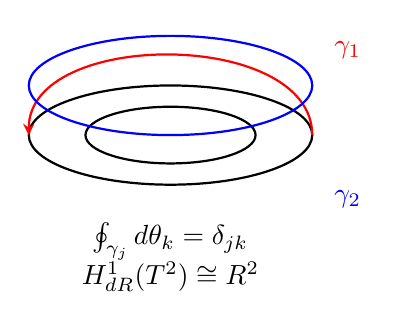
\begin{tikzpicture}[scale=0.9]
  % 环面
  \draw[thick] (0,0) ellipse (2.0 and 0.7);
  \draw[thick] (0,0) ellipse (1.2 and 0.4);
  % 闭合轨道 gamma_1
  \draw[thick, red, ->, >=stealth] (2.0,0) .. controls (2.0,1.5) and (-2.0,1.5) .. (-2.0,0);
  \node[red] at (2.5,1.2) {$\gamma_1$};
  % 闭合轨道 gamma_2
  \draw[thick, blue, ->, >=stealth] (0,0.7) ellipse (2.0 and 0.7);
  \node[blue] at (2.5,-0.9) {$\gamma_2$};
  % 积分符号
  \node at (0,-1.5) {$\oint_{\gamma_j}d\theta_k=\delta_{jk}$};
  \node at (0,-2.0) {$H^1_{dR}(\mathbb{T}^2)\cong\mathbb{R}^2$};
\end{tikzpicture}
\caption{环面上的闭 1-形式与周期积分：$d\theta_j$ 沿 $\gamma_k$ 的积分给出 Kronecker delta。}
\label{fig:period_integral}
\end{figure}

\section{不变环面与可积系统}\label{sec:invariant_torus_periodic}

\begin{remark}[与「流形基础与纤维丛」章的关系]\label{rem:invariant_torus_source}
不变环面的定义已在「流形基础与纤维丛」章 \cref{def:invariant_torus} 给出；本节直接沿用该定义，不重复陈述。
\end{remark}

\begin{theorem}[Liouville--Arnold 定理]\label{thm:liouville_arnold_periodic}
设 $n$ 自由度哈密顿系统具有 $n$ 个独立对合首次积分，且水平集紧致连通。则该水平集微分同胚于 $\mathbb{T}^n$，在其附近存在作用-角坐标 $(I,\theta)$ 使
\[
\omega=\sum_i dI_i\wedge d\theta_i,\qquad \dot I_i=0,\qquad \dot\theta_i=\omega_i(I).
\]
\end{theorem}

\begin{proof}
见 Arnold, \textit{Mathematical Methods of Classical Mechanics}, 2nd ed., Springer, 1989, \S{}49--50。核心思想：$n$ 个对合首次积分生成 $n$ 个可交换的哈密顿流，这些流在紧致水平集上的作用给出 $\mathbb{T}^n$ 结构；作用变量 $I_i$ 由环面上的周期积分定义，角变量 $\theta_i$ 为其共轭。
\end{proof}

\begin{corollary}[周期轨道与准周期轨道的判据]\label{cor:periodic_vs_quasiperiodic}
在不变环面 $\mathbb{T}^n$ 上，轨道 $\theta(t)=\theta_0+\omega t$ 闭合当且仅当各频率成对可公度，即存在 $T>0$ 使 $\omega T\in2\pi\mathbb{Z}^n$（等价地 $\omega_i/\omega_j\in\mathbb{Q}$ 对一切 $i,j$ 成立；若某些 $\omega_j=0$，该分量静止不动，$T$ 取其余分量周期的最小公倍数即可）；否则轨道在 $\mathbb{T}^n$ 上稠密。注意条件不是较弱的“存在 $k\in\mathbb{Z}^n\setminus\{0\}$ 使 $k\cdot\omega=0$”：后者只要求频率在 $\mathbb{Q}$ 上线性相关，例如 $n=3$、$\omega=(1,2,\pi)$ 取 $k=(-2,1,0)$ 即满足，但轨道在 $\mathbb{T}^3$ 上稠密而不闭合。
\end{corollary}

\begin{proof}
闭合性等价于存在 $T>0$ 使 $\omega T\in 2\pi\mathbb{Z}^n$，即 $\omega_i/\omega_j\in\mathbb{Q}$（$\omega_j\ne0$ 时）；$\omega_j=0$ 的分量不贡献周期，$T$ 取其余分量周期的最小公倍数。稠密性由 Kronecker 逼近定理给出。
\end{proof}

\begin{figure}[htbp]
\centering
\begin{tikzpicture}[scale=0.9]

  \draw[thick] (0,0) ellipse (2.0 and 0.7);
  \draw[thick] (0,0) ellipse (1.2 and 0.4);

  \draw[thick, red, ->, >=stealth] (2.0,0) .. controls (2.0,1.5) and (-2.0,1.5) .. (-2.0,0);
  \draw[thick, red, ->, >=stealth] (-2.0,0) .. controls (-2.0,-1.5) and (2.0,-1.5) .. (2.0,0);
  \node[red] at (0,1.8) {成对可公度：闭合};

  \begin{scope}[shift={(6,0)}]
    \draw[thick] (0,0) ellipse (2.0 and 0.7);
    \draw[thick] (0,0) ellipse (1.2 and 0.4);
    \draw[thick, blue] (2.0,0) .. controls (2.0,0.7) and (0.3,0.55) .. (-0.5,0.4)
                                .. controls (-1.3,0.2) and (-1.2,-0.3) .. (-0.2,-0.35)
                                .. controls (0.8,-0.4) and (1.3,-0.1) .. (1.1,0.25)
                                .. controls (0.9,0.55) and (-0.1,0.6) .. (-0.7,0.45);
    \node[blue] at (0,1.8) {不可公度：稠密};
  \end{scope}

\end{tikzpicture}
\caption{不变环面上的轨道闭合判据：频率成对可公度时轨道闭合，不可公度时轨道稠密。}
\label{fig:torus_closure_periodic}
\end{figure}

\section{辛流形与能量面}\label{sec:symplectic_energy}

\begin{definition}[辛流形]\label{def:symplectic_manifold}
$(M,\omega)$ 称为\textbf{辛流形}，若 $M$ 为偶数维光滑流形，$\omega$ 为闭的非退化 2-形式：$d\omega=0$，且对任意 $p\in M$，$\omega_p:T_pM\times T_pM\to\mathbb{R}$ 非退化。
\end{definition}

\begin{definition}[哈密顿向量场]\label{def:hamiltonian_vector_field}
给定 $H\in C^\infty(M)$，\textbf{哈密顿向量场} $X_H$ 由 $\iota_{X_H}\omega=dH$ 唯一确定，即 $\omega(X_H,Y)=dH(Y)$ 对任意 $Y\in\mathfrak{X}(M)$。
\end{definition}

\begin{proposition}[能量面是接触流形]\label{prop:energy_surface_contact}
设 $(M,\omega)$ 为辛流形，$H:M\to\mathbb{R}$，$\Sigma_E=H^{-1}(E)$ 为能量面。若 $dH$ 在 $\Sigma_E$ 上处处非零，则 $\Sigma_E$ 是余维 $1$ 的嵌入子流形，且 $\omega|_{\Sigma_E}$ 的核为 $1$ 维，给出接触结构。
\end{proposition}

\begin{proof}
由正则水平集定理，$\Sigma_E$ 是余维 $1$ 子流形。$\omega|_{\Sigma_E}$ 的核由 $X_H$ 张成（$\iota_{X_H}\omega=dH$，在 $\Sigma_E$ 上 $dH$ 限制为 $0$），故核为 $1$ 维。接触形式可取为 $\alpha=\iota_{X_H}\omega$ 在 $\Sigma_E$ 上的限制。
\end{proof}

\begin{theorem}[Weinstein 猜测（三维已证）]\label{thm:weinstein}
紧致接触流形上的 Reeb 流至少有一条周期轨道。
\end{theorem}

\begin{proof}
\textbf{证明超出本书范围}。这是 Weinstein 猜测：三维情形由 Taubes（2007）证明（Cristofaro-Gardiner--Hutchings（2013）给出后续工作）；一般奇数维仍为公开问题。参见 \cite{weinstein1978}。
\end{proof}

\begin{figure}[htbp]
\centering
\begin{tikzpicture}[scale=0.9]

  \node at (0,3.2) {相空间 $T^*Q$（$2n$ 维）};
  \draw[thick, fill=blue!5] (-3,-1.5) rectangle (3,2.8);

  \draw[thick, red] (-2.5,-0.5) .. controls (-1,2.0) and (1,2.0) .. (2.5,-0.5);
  \node[red] at (2.8,-0.5) {$\Sigma_E=H^{-1}(E)$};
  \node[red] at (-2.7,0.0) {$(2n-1)$ 维};

  \draw[thick, blue, ->, >=stealth] (-1.5,0.5) .. controls (-0.5,1.3) and (0.5,1.3) .. (1.5,0.5);
  \node[blue] at (0,1.7) {周期轨道 $\gamma$};
\end{tikzpicture}
\caption{能量面 $\Sigma_E$ 是相空间中的 $(2n-1)$ 维接触超曲面，周期轨道在其上运动。}
\label{fig:energy_surface_periodic}
\end{figure}

\section{主丛、联络与和乐}\label{sec:principal_bundle_holonomy}

\begin{definition}[主丛]\label{def:principal_bundle}
设 $G$ 为李群，$P$ 为光滑流形，$\pi:P\to M$ 为光滑满射。称 $(P,M,\pi,G)$ 为\textbf{主 $G$-丛}，若 $G$ 自由右作用于 $P$，轨道空间 $P/G$ 微分同胚于 $M$，且局部平凡：对任意 $p\in M$，存在开邻域 $U$ 与 $G$-等变微分同胚 $\Phi:\pi^{-1}(U)\to U\times G$。
\end{definition}

\begin{definition}[联络与和乐]\label{def:connection_holonomy}
主丛 $P\to M$ 上的\textbf{联络}为 $\mathfrak{g}$-值 1-形式 $\mathcal{A}\in\Omega^1(P,\mathfrak{g})$，满足 $\mathcal{A}(X^\#)=X$（$X\in\mathfrak{g}$）与 $R_g^*\mathcal{A}=\operatorname{Ad}_{g^{-1}}\mathcal{A}$。给定闭合轨道 $\gamma:[0,T]\to M$ 与提升 $\tilde\gamma$，\textbf{和乐}为
\[
\operatorname{Hol}_\gamma(\mathcal{A}):=\mathcal{P}\exp\!\left(-\int_0^T\mathcal{A}(\dot{\tilde\gamma}(t))\,dt\right)\in G,
\]
其中 $\mathcal{P}\exp$ 为路径有序指数。和乐仅依赖于 $\gamma$ 的同伦类（当曲率 $\mathcal{F}=d\mathcal{A}+\tfrac12[\mathcal{A},\mathcal{A}]=0$ 时）。
\end{definition}

\begin{proposition}[Wilson 环即和乐]\label{prop:wilson_holonomy}
离散曲率（定义 \ref{def:discrete_curvature}）中的 Wilson 环 $\mathcal{F}_{ij}$ 是主丛联络和乐在 plaquette 上的离散化。当格点间距 $\Delta x\to 0$ 时，$\mathcal{F}_{ij}\to I-i(\Delta x)^2 F_{ij}+O((\Delta x)^3)$，其中 $F_{ij}$ 为连续曲率。
\end{proposition}

\begin{proof}
将联络 $\mathcal{A}$ 在 plaquette 四边上离散化为 $\mathcal{U}_{\mathbf{n},i}=e^{-i\Delta x\mathcal{A}_i}$。由 Baker--Campbell--Hausdorff 公式，四条边的有序乘积展开至二阶给出 $I-i(\Delta x)^2(\partial_i\mathcal{A}_j-\partial_j\mathcal{A}_i-i[\mathcal{A}_i,\mathcal{A}_j])+O((\Delta x)^3)$，方括号内即曲率 $F_{ij}$。
\end{proof}

\begin{figure}[htbp]
\centering
\begin{tikzpicture}[scale=0.9]
  % 格点
  \foreach \x in {0,1,2} {
    \foreach \y in {0,1,2} {
      \node[circle, fill, black, inner sep=1pt] at (\x,\y) {};
    }
  }
  % Plaquette 边
  \draw[->, thick, red, >=stealth] (0.1,0) -- (0.9,0);
  \draw[->, thick, red, >=stealth] (1,0.1) -- (1,0.9);
  \draw[->, thick, red, >=stealth] (0.9,1) -- (0.1,1);
  \draw[->, thick, red, >=stealth] (0,0.9) -- (0,0.1);
  % 标签
  \node[red, below] at (0.5,-0.1) {$\mathcal U_{\mathbf n,i}$};
  \node[red, right] at (1.1,0.5) {$\mathcal U_{\mathbf n+\hat i,j}$};
  \node[red, above] at (0.5,1.1) {$\mathcal U_{\mathbf n+\hat j,i}^\dagger$};
  \node[red, left] at (-0.1,0.5) {$\mathcal U_{\mathbf n,j}^\dagger$};
  \node at (1,-0.8) {Wilson 环 $\mathcal F_{ij}$};
\end{tikzpicture}
\caption{离散曲率（Wilson 环）：plaquette 四条边的幺正算子按序乘积，即主丛联络和乐的离散化。}
\label{fig:wilson_loop}
\end{figure}

\section{周期轨道的模空间}\label{sec:periodic_orbit_moduli}

\begin{definition}[周期轨道模空间]\label{def:periodic_orbit_moduli}
设 $\mathcal{P}(M)$ 为 $M$ 上所有闭合轨道的集合，$\sim$ 为时间平移与重参数化等价关系。\textbf{周期轨道模空间}为 $\mathcal{M}_{\text{per}}(M):=\mathcal{P}(M)/\sim$。当 $M$ 为辛流形时，$\mathcal{M}_{\text{per}}$ 可赋予自然辛结构或接触结构。
\end{definition}

\begin{proposition}[模空间的切空间]\label{prop:moduli_tangent}
设 $\gamma$ 为非退化周期轨道，Floquet 乘子为 $\rho_1,\dots,\rho_n$。则 $\mathcal{M}_{\text{per}}$ 在 $[\gamma]$ 处的切空间维数为 $\#\{|\rho_i|=1\}$（中心方向的个数）。
\end{proposition}

\begin{proof}
由 Floquet 理论，$\gamma$ 附近的线性化动力学分解为稳定、不稳定、中心三个子空间。模空间的形变仅沿中心方向（不指数趋近或远离 $\gamma$ 的方向）进行，故切空间维数等于中心方向个数。
\end{proof}



\begin{figure}[htbp]
\centering
\begin{tikzpicture}[scale=0.9]
  % 各类格
  \foreach \x/\y/\ang in {-3.5/1.0/0, -2.2/1.0/20, -0.9/1.0/-30, 0.4/1.0/45} {
    \begin{scope}[shift={(\x,\y)}, rotate=\ang]
      \draw[thick] (0,0) -- (0.7,0);
      \draw[thick] (0,0) -- (0.3,0.6);
      \draw[thick, dashed] (0.7,0) -- (1.0,0.6);
      \draw[thick, dashed] (0.3,0.6) -- (1.0,0.6);
    \end{scope}
  }
  \node at (-1.6,1.9) {周期格族};
  \draw[->, thick, >=stealth] (0.8,0.5) -- (2.0,0.5);
  \draw[thick, fill=green!10] (2.4,-0.5) rectangle (5.4,1.5);
  \node at (3.9,1.8) {模空间 $SL(2,\mathbb Z)\setminus\mathbb H$};
  \node at (3.9,0.5) {$\tau$};
  \node at (3.9,-0.2) {等价类};
\end{tikzpicture}
\caption{模空间作为周期结构的分类空间：等价类被 $\tau$ 参数化。}
\label{fig:moduli_space_periodic}
\end{figure}

\section{离散格点流形的基本结构}\label{sec:discrete_lattice}

\begin{axiom}[离散性本原公理]\label{axm:discreteness}
空间和时间的基本结构是\textbf{离散格点}。连续统不是基本的存在，而是通过对离散格点进行\textbf{无限次微分}（在空间上）或\textbf{无限次积分}（在时间上）得到的极限近似。具体而言：
\begin{enumerate}[label=(\roman*)]
    \item 空间由离散格点构成，格点间距 $\Delta x>0$ 是空间的最小分辨率。
    \item 时间由离散时刻 $t_m=m\Delta t$（$m\in\mathbb{N}$）构成。
    \item 任何“连续函数”是格点上离散函数在无限加密极限下的近似。
    \item 分辨率 $\Delta x,\Delta t$ 由观察系统的参数决定。
\end{enumerate}
\end{axiom}

\begin{definition}[离散时空格点]\label{def:discrete_spacetime_lattice}
离散时空格点为 $\mathcal{L}=\mathcal{L}_{\text{space}}\times\{t_m:m\in\mathbb{N}\}$。格点间距 $\Delta x$ 和 $\Delta t$ 由观察系统参数决定：
\[
\Delta x=\frac{1}{R_0}\cdot\frac{r^2+\sigma}{\sigma},\quad \Delta t=\frac{N_0}{R_0}\cdot\frac{r^2+\sigma}{\sigma}.
\]
\end{definition}

\begin{proposition}[格点间距与观察者尺度的关系]\label{prop:lattice_spacing_observer}
格点间距 $\Delta x$ 是观察者尺度 $\sigma$ 的严格递减函数：
\[
\frac{\partial(\Delta x)}{\partial\sigma}=-\frac{1}{R_0}\cdot\frac{r^2}{\sigma^2}<0\quad(r>0).
\]
\end{proposition}

\begin{proof}
由定义 \ref{def:discrete_spacetime_lattice}，$\Delta x=\frac{1}{R_0}(r^2/\sigma+1)$。对 $\sigma$ 求偏导数得 $\partial(\Delta x)/\partial\sigma=-r^2/(R_0\sigma^2)<0$。
\end{proof}

\begin{definition}[三种势矢量]\label{def:three_potential_vectors}
在离散时空格点上，每个格点存储三种势矢量：
\begin{enumerate}[label=(\roman*)]
    \item \textbf{空间势} $\mathbf{V}_S$：由旋度驱动，$|\mathbf{V}_S|^2$ 对应质量密度；
    \item \textbf{时间势} $\mathbf{V}_T$：由梯度驱动，$|\mathbf{V}_T|^2$ 对应能量密度；
    \item \textbf{观察势} $\mathbf{V}_P$：由散度驱动，$|\mathbf{V}_P|^2$ 对应观察者尺度 $\sigma$。
\end{enumerate}
\end{definition}

\section{格点上的三种基本操作}\label{sec:lattice_operations}

\begin{definition}[格点平移操作]\label{def:lattice_translation}
平移操作 $\mathcal{T}_{\mathbf{m}}$ 将势矢量从格点 $\mathbf{x}_{\mathbf{n}}$ 移动到 $\mathbf{x}_{\mathbf{n}+\mathbf{m}}$：$\mathcal{T}_{\mathbf{m}}\cdot\mathbf{V}(\mathbf{x}_{\mathbf{n}})=\mathbf{V}(\mathbf{x}_{\mathbf{n}+\mathbf{m}})$。平移保持矢量的模长和方向不变。
\end{definition}

\begin{definition}[格点缩放操作]\label{def:lattice_scaling}
缩放操作 $\mathcal{S}_\alpha$ 改变势矢量的模长：$\mathcal{S}_\alpha\cdot\mathbf{V}=\alpha\mathbf{V}$。缩放以比例因子改变矢量的模长，保持方向不变。
\end{definition}

\begin{definition}[格点旋转操作]\label{def:lattice_rotation}
旋转操作 $\mathcal{R}_\theta$ 改变势矢量的方向，保持模长不变。
\end{definition}

\begin{figure}[htbp]
\centering
\begin{tikzpicture}[scale=0.9]
  \begin{scope}[shift={(-5,0)}]
    \draw[->, thick, blue, >=stealth] (0,0) -- (1.0,0);
    \draw[->, thick, blue, >=stealth] (2.0,0) -- (3.0,0);
    \node at (0.5,-0.5) {$\mathcal T_{\mathbf m}$};
    \node at (1.5,0.3) {平移};
    \draw[->, thick, red, >=stealth] (0.5,-0.8) -- (2.5,-0.8);
    \node at (1.5,-1.1) {位置改变};
  \end{scope}
  \begin{scope}[shift={(0,0)}]
    \draw[->, thick, blue, >=stealth] (0,0) -- (1.0,0);
    \draw[->, thick, blue, >=stealth] (0,0) -- (1.8,0);
    \node at (0.5,-0.5) {$\mathcal S_\alpha$};
    \node at (1.5,0.3) {缩放};
    \node at (0.9,-1.1) {模长改变};
  \end{scope}
  \begin{scope}[shift={(5,0)}]
    \draw[->, thick, blue, >=stealth] (0,0) -- (1.0,0);
    \draw[->, thick, blue, >=stealth] (0,0) -- (0.7,0.7);
    \node at (0.5,-0.5) {$\mathcal R_\theta$};
    \node at (1.5,0.3) {旋转};
    \node at (0.9,-1.1) {方向改变};
  \end{scope}
\end{tikzpicture}
\caption{三种基本操作：平移改变位置，缩放改变模长，旋转改变方向。}
\label{fig:lattice_operations}
\end{figure}

\begin{proposition}[三种操作的不可互约性]\label{prop:lattice_operations_irreducibility}
平移、缩放、旋转三种操作彼此独立，互不约化。任何格点上的势矢量演化都可分解为这三种基本操作的复合。
\end{proposition}

\begin{proof}
平移只改变位置（不触及模长与方向），缩放只改变模长（不触及位置与方向），旋转只改变方向（不触及位置与模长）。三者作用于互不重叠的自由度，任一个不能由其余两个复合得到。任一格点状态的演化可分解为 $\mathcal{R}_\theta\circ\mathcal{S}_\alpha\circ\mathcal{T}_{\mathbf{m}}$ 的复合。
\end{proof}

\begin{theorem}[三种操作在离散格点上的守恒律]\label{thm:lattice_three_conservation}
\begin{enumerate}[label=(\roman*)]
    \item 平移操作的守恒量——动量：$|\mathcal{T}_{\mathbf{m}}\cdot\mathbf{V}|^2=|\mathbf{V}|^2$。
    \item 旋转操作的守恒量——角动量：$|\mathcal{R}_\theta\cdot\mathbf{V}|^2=|\mathbf{V}|^2$。
    \item 缩放操作的守恒量——标度荷：$\alpha=1$ 时 $|\mathcal{S}_\alpha\cdot\mathbf{V}|^2=|\mathbf{V}|^2$；标度荷守恒等价于 $\nabla_{\Delta}\cdot\mathbf{V}_P=0$。
\end{enumerate}
\end{theorem}

\begin{proof}
(i) 平移不改变矢量本身。(ii) 旋转矩阵是正交矩阵。(iii) $\alpha=1$ 时 $\mathcal{S}_1$ 是恒等映射。
\end{proof}

\section{三大微分算子的严格理论}\label{sec:three_operators_strict}

\subsection{连续情形：内蕴定义}

\begin{definition}[梯度——内蕴定义]\label{def:gradient_intrinsic}
设 $(M,g)$ 为 $n$ 维黎曼流形，$f\in C^\infty(M)$。$f$ 的\textbf{梯度} $\nabla f$ 是由 $g_p(\nabla f(p),v)=df_p(v)$（$\forall v\in T_pM$）唯一确定的向量场。
\end{definition}

\begin{proposition}[梯度的坐标公式]\label{prop:gradient_coordinate}
在局部坐标 $(x^1,\dots,x^n)$ 下，$\nabla f=\sum_{i,j}g^{ij}\frac{\partial f}{\partial x^i}\frac{\partial}{\partial x^j}$，其中 $(g^{ij})$ 是 $(g_{ij})$ 的逆矩阵。
\end{proposition}

\begin{proof}
设 $\nabla f=\sum_i a^i\frac{\partial}{\partial x^i}$。由 $g(\nabla f,v)=df(v)$ 对任意 $v$ 成立，取 $v=\frac{\partial}{\partial x^k}$ 得 $\sum_i a^i g_{ik}=\frac{\partial f}{\partial x^k}$。两边乘以 $g^{jk}$ 并对 $k$ 求和，利用 $\sum_k g_{ik}g^{jk}=\delta_i^j$ 得 $a^j=\sum_k g^{jk}\frac{\partial f}{\partial x^k}$。
\end{proof}

\begin{definition}[散度——内蕴定义]\label{def:divergence_intrinsic}
设 $(M,g)$ 为 $n$ 维定向黎曼流形，$X$ 为光滑向量场，$d\mu$ 为黎曼体积形式。$X$ 的\textbf{散度} $\nabla\cdot X$ 由 $\mathcal{L}_X(d\mu)=(\nabla\cdot X)d\mu$ 定义。
\end{definition}

\begin{proposition}[散度的坐标公式]\label{prop:divergence_coordinate}
在局部坐标下，$\nabla\cdot X=\frac{1}{\sqrt{\det g}}\sum_i\frac{\partial}{\partial x^i}(\sqrt{\det g}\,X^i)$。在欧氏空间中退化为 $\nabla\cdot X=\sum_i\frac{\partial X^i}{\partial x^i}$。
\end{proposition}

\begin{proof}
由 Cartan 公式 $\mathcal{L}_X=d\circ\iota_X+\iota_X\circ d$ 与 $d(d\mu)=0$ 得 $\mathcal{L}_X(d\mu)=d(\iota_X d\mu)$。在局部坐标下计算即得。
\end{proof}

\begin{definition}[旋度——内蕴定义]\label{def:curl_intrinsic}
设 $(M,g)$ 为 $3$ 维定向黎曼流形，$X$ 为光滑向量场。$X$ 的\textbf{旋度}由 $(\nabla\times X)^\flat=\star(dX^\flat)$ 定义，其中 $X^\flat$ 是度量对偶 1-形式，$\star$ 是霍奇星算子。
\end{definition}

\begin{proposition}[旋度的坐标公式]\label{prop:curl_coordinate}
在欧氏空间 $\mathbb{R}^3$ 中，$\nabla\times\mathbf{F}=(\partial_2F_3-\partial_3F_2,\partial_3F_1-\partial_1F_3,\partial_1F_2-\partial_2F_1)$。
\end{proposition}

\begin{proof}
由 $dF^\flat=(\partial_2F_3-\partial_3F_2)dx^2\wedge dx^3+\cdots$，取霍奇星并提升指标即得。
\end{proof}

\begin{proposition}[三大算子的恒等式]\label{prop:three_operator_identities}
在 $3$ 维欧氏空间中，$\nabla\times(\nabla f)=\mathbf{0}$，$\nabla\cdot(\nabla\times\mathbf{F})=0$。
\end{proposition}

\begin{proof}
$(\nabla\times\nabla f)^\flat=\star d(df)=\star\cdot 0=0$；$\nabla\cdot(\nabla\times\mathbf{F})=\star^{-1}d\star(\star dF^\flat)=\star^{-1}d^2F^\flat=0$。
\end{proof}

\subsection{离散情形：严格定义与推导}

\begin{definition}[离散梯度]\label{def:discrete_gradient_strict}
设 $f$ 为格点上的光滑标量场。中心差分为 $(\Delta_i^cf)(\mathbf{x}_{\mathbf{n}}):=\frac{f(\mathbf{x}_{\mathbf{n}}+\Delta x\hat{\mathbf{e}}_i)-f(\mathbf{x}_{\mathbf{n}}-\Delta x\hat{\mathbf{e}}_i)}{2\Delta x}$。\textbf{离散梯度}为 $(\nabla_{\Delta}f)(\mathbf{x}_{\mathbf{n}}):=((\Delta_1^cf)(\mathbf{x}_{\mathbf{n}}),\dots,(\Delta_d^cf)(\mathbf{x}_{\mathbf{n}}))$。
\end{definition}

\begin{proposition}[离散梯度的误差估计]\label{prop:discrete_gradient_error}
设 $f\in C^3$，则 $(\Delta_i^cf)(\mathbf{x})=\frac{\partial f}{\partial x^i}(\mathbf{x})+\frac{(\Delta x)^2}{6}\frac{\partial^3f}{\partial(x^i)^3}(\mathbf{x})+O((\Delta x)^4)$。
\end{proposition}

\begin{proof}
对 $f(\mathbf{x}\pm\Delta x\hat{\mathbf{e}}_i)$ 作泰勒展开，两式相减消去偶数阶项，除以 $2\Delta x$ 即得。
\end{proof}

\begin{definition}[离散散度]\label{def:discrete_divergence_strict}
$(\nabla_{\Delta}\cdot\mathbf{V})(\mathbf{x}_{\mathbf{n}}):=\sum_{i=1}^d(\Delta_i^cV_i)(\mathbf{x}_{\mathbf{n}})$。
\end{definition}

\begin{proposition}[离散散度的通量解释]\label{prop:discrete_divergence_flux}
$(\nabla_{\Delta}\cdot\mathbf{V})(\mathbf{x}_{\mathbf{n}})\cdot(\Delta x)^d=\sum_{i=1}^d[V_i(\mathbf{x}_{\mathbf{n}}+\tfrac{\Delta x}{2}\hat{\mathbf{e}}_i)-V_i(\mathbf{x}_{\mathbf{n}}-\tfrac{\Delta x}{2}\hat{\mathbf{e}}_i)](\Delta x)^{d-1}+O((\Delta x)^{d+1})$。
\end{proposition}

\begin{proof}
将中心差分中的值用中点值泰勒展开并整理即得。
\end{proof}

\begin{definition}[离散旋度]\label{def:discrete_curl_strict}
$(\nabla_{\Delta}\times\mathbf{V})(\mathbf{x}_{\mathbf{n}}):=((\Delta_2^cV_3-\Delta_3^cV_2)(\mathbf{x}_{\mathbf{n}}),(\Delta_3^cV_1-\Delta_1^cV_3)(\mathbf{x}_{\mathbf{n}}),(\Delta_1^cV_2-\Delta_2^cV_1)(\mathbf{x}_{\mathbf{n}}))$。
\end{definition}

\begin{proposition}[离散旋度的环量解释]\label{prop:discrete_curl_circulation}
$(\nabla_{\Delta}\times\mathbf{V})_k(\mathbf{x}_{\mathbf{n}})=\frac{1}{(\Delta x)^2}\oint_{C_k}\mathbf{V}\cdot d\mathbf{l}+O(\Delta x)$。
\end{proposition}

\begin{proof}
以 $k=3$ 为例，用中心差分近似 plaquette 四条边的积分并除以面积。
\end{proof}

\begin{proposition}[离散恒等式的精确成立]\label{prop:discrete_exact_identities}
在任意有限 $\Delta x>0$ 下，$\nabla_{\Delta}\times(\nabla_{\Delta}f)=\mathbf{0}$，$\nabla_{\Delta}\cdot(\nabla_{\Delta}\times\mathbf{V})=0$。
\end{proposition}

\begin{proof}
中心差分算子可交换（$\Delta_i^c\Delta_j^c=\Delta_j^c\Delta_i^c$），展开后逐项精确相消。
\end{proof}

\subsection{积分定理}

\begin{theorem}[Stokes 定理——流形版本]\label{thm:stokes_manifold}
设 $M$ 为 $n$ 维定向光滑流形，$\Omega\subseteq M$ 为 $(n-1)$ 维定向带边子流形，$\omega$ 为 $(n-1)$ 形式，则 $\int_\Omega d\omega=\oint_{\partial\Omega}\omega$。
\end{theorem}

\begin{proof}
\textbf{证明要点}（完整证明见 \cite{lee2012smooth} \S{}16）。分三步。\emph{(i) 局部化}：由单位分解，只需在每个坐标卡内证明；再经坐标拉回，归约为上半空间 $\mathbb{H}^n=\{x_n\ge0\}$ 上紧支集形式的情形。\emph{(ii) 上半空间情形}：写 $\omega=\sum_{i=1}^{n}f_i\,dx_1\wedge\cdots\wedge\widehat{dx_i}\wedge\cdots\wedge dx_n$，则 $d\omega=\sum_{i=1}^{n}(-1)^{i-1}\partial_i f_i\,dx_1\wedge\cdots\wedge dx_n$。由 Fubini 定理先对 $x_i$ 积分，并用微积分基本定理：当 $i<n$ 时 $f_i$ 在 $x_i$ 方向紧支集，积分为零；当 $i=n$ 时仅边界 $\{x_n=0\}$ 留下贡献，得 $\int_{\mathbb{H}^n}\partial_n f_n\,dx=-\int_{\partial\mathbb{H}^n}f_n$（负号来自外法向指向 $-x_n$）。\emph{(iii) 拼接}：把局部恒等式按单位分解求和，内部公共面上的诱导定向相反，贡献两两相消，只剩 $\partial\Omega$ 上的积分，即得 $\int_\Omega d\omega=\oint_{\partial\Omega}\omega$。
\end{proof}

\begin{theorem}[Gauss 散度定理——流形版本]\label{thm:gauss_divergence_manifold}
设 $(M,g)$ 为 $n$ 维定向黎曼流形，$\Omega\subseteq M$ 紧致，$\partial\Omega$ 光滑，$\mathbf{n}$ 为外法向量场，则 $\int_\Omega(\nabla\cdot X)d\mu=\oint_{\partial\Omega}g(X,\mathbf{n})dS$。
\end{theorem}

\begin{proof}
由 $\mathcal{L}_X(d\mu)=(\nabla\cdot X)d\mu$ 和 Stokes 定理，$\int_\Omega(\nabla\cdot X)d\mu=\oint_{\partial\Omega}\iota_Xd\mu$，边界项限制为 $g(X,\mathbf{n})dS$。
\end{proof}

\begin{corollary}[Green 恒等式]\label{cor:green_identity}
$\int_\Omega(f\nabla^2h+g(\nabla f,\nabla h))d\mu=\oint_{\partial\Omega}f\,g(\nabla h,\mathbf{n})dS$。
\end{corollary}

\begin{proof}
取 $X=f\nabla h$，应用 Gauss 散度定理并展开散度。
\end{proof}

\begin{proposition}[离散 Green 公式与离散散度定理]\label{prop:discrete_green_divergence}
在离散格点上，$\sum_{\mathbf{n}\in V}(\nabla_{\Delta}\cdot\mathbf{V})(\mathbf{x}_{\mathbf{n}})(\Delta x)^d=\sum_{\partial V}\mathbf{V}\cdot\mathbf{n}(\Delta x)^{d-1}$，在任意有限 $\Delta x$ 下精确成立。
\end{proposition}

\begin{proof}
内部边被两个相邻元胞以相反方向各计一次，精确相消；仅边界贡献保留。
\end{proof}

\subsection{连续极限的完整证明}

\begin{theorem}[连续极限定理——完整版]\label{thm:continuum_limit_full}
设 $f\in C^3$，$\mathbf{V}\in C^3$。在 $\Delta x\to 0$ 下：
\begin{enumerate}[label=(\roman*)]
    \item $\lim\nabla_{\Delta}f=\nabla f$，误差 $O((\Delta x)^2)$；
    \item $\lim\nabla_{\Delta}\cdot\mathbf{V}=\nabla\cdot\mathbf{V}$，误差 $O((\Delta x)^2)$；
    \item $\lim\nabla_{\Delta}\times\mathbf{V}=\nabla\times\mathbf{V}$，误差 $O((\Delta x)^2)$；
    \item 对任意有限 $\Delta t$，$\mathcal{U}_{\Delta}^N=e^{-i\mathcal{H}t}$ 精确成立（$N=t/\Delta t$）；
    \item $\lim\mathcal{F}_{ij}=I-i(\Delta x)^2F_{ij}+O((\Delta x)^3)$。
\end{enumerate}
\end{theorem}

\begin{proof}
(i) 由命题 \ref{prop:discrete_gradient_error}。(ii) 对每个分量应用 (i)。(iii) 离散旋度是 $\Delta_i^cV_j$ 的线性组合。(iv) $\mathcal{U}_{\Delta}=e^{-i\Delta t\mathcal{H}}$，$N$ 次迭代得 $e^{-i\mathcal{H}t}$。(v) 由命题 \ref{prop:discrete_continuous_curvature}。
\end{proof}

\section{离散幺正理论}\label{sec:discrete_unitary_theory}

\begin{definition}[离散幺正算子]\label{def:discrete_unitary}
格点 $\mathbf{x}_{\mathbf{n}}$ 上的\textbf{离散幺正算子} $\mathcal{U}_{\mathbf{n}}$ 满足 $\mathcal{U}_{\mathbf{n}}^\dagger\mathcal{U}_{\mathbf{n}}=I_d$。势矢量演化：$\mathbf{V}(t_{m+1})=\mathcal{U}_{\mathbf{n}}\mathbf{V}(t_m)$。
\end{definition}

\begin{proposition}[幺正性与模方守恒]\label{prop:unitary_norm_conservation}
$|\mathbf{V}(t_{m+1})|^2=|\mathbf{V}(t_m)|^2$。
\end{proposition}

\begin{proof}
$|\mathcal{U}\mathbf{V}|^2=(\mathcal{U}\mathbf{V})^\dagger(\mathcal{U}\mathbf{V})=\mathbf{V}^\dagger\mathcal{U}^\dagger\mathcal{U}\mathbf{V}=\mathbf{V}^\dagger\mathbf{V}=|\mathbf{V}|^2$。
\end{proof}

\begin{proposition}[幺正演化与格点总能量守恒]\label{prop:unitary_total_energy}
$E_{\text{total}}=\sum_{\mathbf{n}}|\mathbf{V}_{\mathbf{n}}|^2$ 在演化中守恒。
\end{proposition}

\begin{proof}
每个格点模方独立守恒，求和即得。
\end{proof}

\begin{proposition}[幺正性与三种守恒律的对应]\label{prop:unitary_conservation_laws}
能量守恒、角动量守恒、标度不变性。
\end{proposition}

\begin{proof}
(i) 由命题 \ref{prop:unitary_norm_conservation}。(ii) $|\mathbf{V}_S\times\mathcal{R}_\theta\mathbf{V}_S|=|\mathbf{V}_S|^2|\sin\theta|$。(iii) $\nabla_{\Delta}\cdot\mathbf{V}_P=0$ 时演化算子为纯旋转。
\end{proof}

\begin{corollary}[离散幺正演化与 Noether 定理]\label{cor:unitary_noether}
离散守恒律不依赖于 $\Delta t\to 0$ 的极限。
\end{corollary}

\begin{proof}
由命题 \ref{prop:unitary_conservation_laws} 直接得出。
\end{proof}

\begin{figure}[htbp]
\centering
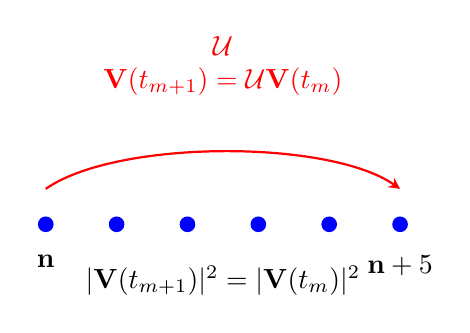
\begin{tikzpicture}[scale=0.9]
  \foreach \x in {0,1,2,3,4,5} {
    \node[circle, fill, blue, inner sep=2pt] (n\x) at (\x,0) {};
  }
  \node[below] at (0,-0.3) {$\mathbf n$};
  \node[below] at (5,-0.3) {$\mathbf n+5$};
  \draw[->, thick, red, >=stealth] (0,0.5) .. controls (1,1.2) and (4,1.2) .. (5,0.5);
  \node[red, yshift=1cm] at (2.5,1.4) {$\mathcal U$};
  \node[red, yshift=1cm] at (2.5,0.9) {$\mathbf V(t_{m+1})=\mathcal U\mathbf V(t_m)$};
  \node at (2.5,-0.8) {$|\mathbf V(t_{m+1})|^2=|\mathbf V(t_m)|^2$};
\end{tikzpicture}
\caption{离散幺正演化：格点上的势矢量经幺正算子作用后模方守恒。}
\label{fig:discrete_unitary}
\end{figure}

\begin{definition}[离散幺正演化的生成元]\label{def:unitary_generator}
$\mathcal{U}_{\mathbf{n}}=e^{-i\Delta t\mathcal{H}_{\mathbf{n}}}$，$\mathcal{H}_{\mathbf{n}}$ 为厄米矩阵。
\end{definition}

\begin{proposition}[生成元的厄米性与演化算子的幺正性等价]\label{prop:generator_hermitian}
$\mathcal{U}=e^{-i\Delta t\mathcal{H}}$ 幺正当且仅当 $\mathcal{H}$ 厄米。
\end{proposition}

\begin{proof}
（$\Leftarrow$）$\mathcal{U}^\dagger\mathcal{U}=e^{i\Delta t\mathcal{H}^\dagger}e^{-i\Delta t\mathcal{H}}=I$。（$\Rightarrow$）$\mathcal{U}$ 幺正 $\Rightarrow$ 谱在单位圆上 $\Rightarrow$ $\mathcal{H}$ 谱为实数，且 $\mathcal{U}^\dagger=\mathcal{U}^{-1}=e^{i\Delta t\mathcal{H}}$，故 $\mathcal{H}^\dagger=\mathcal{H}$。
\end{proof}

\begin{proposition}[离散幺正算子的谱结构]\label{prop:discrete_unitary_spectrum}
离散幺正算子 $\mathcal{U}$ 的所有本征值 $\lambda$ 满足 $|\lambda|=1$。
\end{proposition}

\begin{proof}
$\mathcal{U}\mathbf{v}=\lambda\mathbf{v}$，$\|\mathbf{v}\|^2=\|\mathcal{U}\mathbf{v}\|^2=|\lambda|^2\|\mathbf{v}\|^2$，故 $|\lambda|=1$。
\end{proof}

\begin{proposition}[离散幺正算子与 Floquet 理论]\label{prop:discrete_unitary_floquet}
离散幺正算子 $\mathcal{U}$ 可视为 Floquet 算子。其本征值 $e^{-i\varepsilon}$ 对应准能量 $\varepsilon$，在 Floquet–Brillouin 区 $[-\pi,\pi)$ 内唯一确定。
\end{proposition}

\begin{proof}
由 $\mathcal{U}=e^{-i\Delta t\mathcal{H}}$，本征值 $e^{-i\varepsilon}$ 对应 $\varepsilon=\Delta t\cdot E$。由于 $e^{-i\varepsilon}$ 以 $2\pi$ 为周期，$\varepsilon$ 仅在模 $2\pi$ 意义下确定。
\end{proof}

\begin{figure}[htbp]
\centering
\begin{tikzpicture}[scale=0.9]
  \draw[thick] (0,0) circle (1.5);
  \draw[->, thick, >=stealth] (-1.8,0) -- (1.8,0);
  \draw[->, thick, >=stealth] (0,-1.8) -- (0,1.8);
  \foreach \a in {0,45,90,135,180,225,270,315} {
    \node[circle, fill, red, inner sep=1.5pt] at (\a:1.5) {};
  }
  \node[red] at (1.8,1.8) {$\lambda=e^{i\theta}$};
  \node at (0,-2.2) {$|\lambda|=1$：本征值在单位圆上};
  \node at (2.5,0.5) {$\theta=-\varepsilon$};
  \node[xshift=1cm] at (2.5,-0.5) {$\varepsilon\in[-\pi,\pi)$};
\end{tikzpicture}
\caption{离散幺正算子的谱：本征值全部位于单位圆上，对应准能量在 Floquet–Brillouin 区内。}
\label{fig:unitary_spectrum}
\end{figure}

\begin{proposition}[离散幺正算子的周期条件]\label{prop:discrete_period_condition}
$\mathcal{U}^p=I$ 当且仅当所有本征值是 $p$ 次单位根。
\end{proposition}

\begin{proof}
$\mathcal{U}^p=I$ 等价于 $\mathcal{U}$ 的所有本征值的 $p$ 次幂为 $1$。
\end{proof}

\begin{corollary}[周期性与准能量的有理相关性]\label{cor:period_quasienergy}
$\mathcal{U}$ 具有周期 $p$ 当且仅当所有准能量 $\varepsilon_j$ 满足 $\varepsilon_j\in\frac{2\pi}{p}\mathbb{Z}$（模 $2\pi$）。
\end{corollary}

\begin{proof}
由 $\lambda_j=e^{-i\varepsilon_j}$ 与 $\lambda_j^p=1$ 得 $e^{-ip\varepsilon_j}=1$，即 $p\varepsilon_j\in 2\pi\mathbb{Z}$。
\end{proof}

\begin{proposition}[离散时间量子行走的演化算子]\label{prop:dtqw_evolution}
离散时间量子行走的演化由周期幺正算子 $\mathcal{U}=SR$ 支配，其中 $S$ 是硬币态依赖的移位算子，$R$ 是硬币算子。$m$ 步后的状态为 $|\Psi_m\rangle=(SR)^m|\Psi_0\rangle$。
\end{proposition}

\begin{proof}
这是离散时间量子行走的标准定义。$S$ 和 $R$ 均为幺正算子，其乘积 $SR$ 亦幺正。位置无关的硬币算子与周期边界条件给出平移对称性，从而可通过傅里叶变换将 $S$ 对角化。
\end{proof}

\begin{proposition}[离散幺正演化与离散流守恒]\label{prop:discrete_current_conservation}
离散幺正演化保持离散概率流守恒：$\partial_t\rho_n+\sum_i\Delta_i^cj_{n,i}=0$，其中 $\rho_n=|\Psi_n|^2$ 是格点概率密度。
\end{proposition}

\begin{proof}
由幺正演化 $|\Psi_{m+1}\rangle=\mathcal{U}|\Psi_m\rangle$，概率密度满足 $\rho_{m+1,n}-\rho_{m,n}=\langle\Psi_m|\mathcal{U}^\dagger P_n\mathcal{U}-P_n|\Psi_m\rangle$，对于局部幺正算子可写成相邻格点流之差。
\end{proof}

\begin{example}[格点上的二阶周期振荡]\label{ex:lattice_c2}
$\mathcal{U}=-I$，$\mathcal{U}^2=I$。
\end{example}

\begin{example}[格点上的 $C_4$ 旋转周期]\label{ex:lattice_c4}
$\mathcal{U}=R_{\pi/2}$，$\mathcal{U}^4=I$。
\end{example}

\section{离散曲率}\label{sec:discrete_curvature}

\begin{definition}[格点上的最小闭合回路]\label{def:plaquette}
二维正方格点上的 plaquette 由四条边组成。
\end{definition}

\begin{definition}[离散曲率——Wilson 环]\label{def:discrete_curvature}
$\mathcal{F}_{ij}=\mathcal{U}_{\mathbf{n},i}\mathcal{U}_{\mathbf{n}+\hat{\mathbf{e}}_i,j}\mathcal{U}_{\mathbf{n}+\hat{\mathbf{e}}_j,i}^\dagger\mathcal{U}_{\mathbf{n},j}^\dagger$。
\end{definition}

\begin{proposition}[离散曲率的幺正性]\label{prop:wilson_unitary}
$\mathcal{F}_{ij}^\dagger\mathcal{F}_{ij}=I$。
\end{proposition}

\begin{proof}
直接验证，利用各边算子的幺正性。
\end{proof}

\begin{proposition}[离散曲率与连续曲率的关系]\label{prop:discrete_continuous_curvature}
$\mathcal{F}_{ij}=I-i(\Delta x)^2F_{ij}+O((\Delta x)^3)$。
\end{proposition}

\begin{proof}
泰勒展开并应用 Baker–Campbell–Hausdorff 公式。
\end{proof}

\begin{lemma}[Wilson 环的同伦不变性]\label{ch12_wilson_homotopy_lemma}
平坦区域内，可收缩回路的 Wilson 环为 $I$，且 Wilson 环只依赖于同伦类。
\end{lemma}

\begin{proof}
对回路内部全部 plaquette 的 Wilson 环取乘积，内部边逐边相消，仅边界贡献保留。
\end{proof}

\begin{corollary}[平坦连接的全局相位锁定]\label{ch12_wilson_flat_corollary}
全部 plaquette 平坦时，任意闭合回路的 Wilson 环为 $I$。
\end{corollary}

\begin{proof}
由引理 \ref{ch12_wilson_homotopy_lemma} 直接得出。
\end{proof}

\begin{lemma}[环面 Wilson 环乘积恒等式]\label{ch12_gauss_bonnet_lemma}
环面上全部 plaquette 的 Wilson 环之积等于 $1$。
\end{lemma}

\begin{proof}
每条边恰属于两个 plaquette，以相反方向各出现一次，逐边相消。
\end{proof}

\begin{corollary}[离散通量量子化]\label{ch12_gauss_bonnet_corollary}
总相位 $\sum\theta_{\mathbf{n}}\in 2\pi\mathbb{Z}$。
\end{corollary}

\begin{proof}
由引理 \ref{ch12_gauss_bonnet_lemma} 直接得出。
\end{proof}

\section{守恒律在周期流形上的体现}\label{sec:conservation_periodic_manifolds}

\begin{proposition}[格点上的能量守恒]\label{prop:lattice_energy_conservation}
$E_{\mathbf{n}}=|\mathbf{V}_T|^2$ 在演化中精确守恒。
\end{proposition}

\begin{proof}
由命题 \ref{prop:unitary_norm_conservation} 直接得出。
\end{proof}

\begin{proposition}[格点上的角动量守恒]\label{prop:lattice_angular_momentum_conservation}
$L_{\mathbf{n}}$ 守恒当且仅当旋转角为常数。
\end{proposition}

\begin{proof}
$L_{\mathbf{n}}=|\mathbf{V}_S|^2|\sin\theta|$，模方守恒保证结论。
\end{proof}

\begin{proposition}[格点上的标度不变性]\label{prop:lattice_scale_invariance}
标度不变性等价于 $\nabla_{\Delta}\cdot\mathbf{V}_P=0$。
\end{proposition}

\begin{proof}
无净缩放通量时演化算子为纯旋转，模方守恒。
\end{proof}

\begin{theorem}[守恒律在三种周期流形上的统一]\label{thm:conservation_periodic_manifolds}
平移周期流形（动量守恒）、旋转周期流形（角动量守恒）、缩放周期流形（标度荷守恒）。
\end{theorem}

\begin{proof}
由命题 \ref{prop:lattice_energy_conservation}、\ref{prop:lattice_angular_momentum_conservation}、\ref{prop:lattice_scale_invariance} 逐条对应。
\end{proof}

\begin{figure}[htbp]
\centering
\begin{tikzpicture}[
  box/.style={draw, rounded corners, align=center, inner sep=5pt, font=\small},
  arr/.style={->, thick, >=stealth}
]
  \node[box, fill=blue!8] (trans) {平移周期流形\\动量守恒};
  \node[box, fill=orange!12, right=1.0cm of trans] (rot) {旋转周期流形\\角动量守恒};
  \node[box, fill=green!12, right=1.0cm of rot] (scale) {缩放周期流形\\标度荷守恒};
  \node[box, fill=red!8, below=1.2cm of $(trans)!0.5!(scale)$] (unity) {离散格点 + 具有周期轨道的群 + 算子结构};
  \draw[arr] (trans) -- (unity);
  \draw[arr] (rot) -- (unity);
  \draw[arr] (scale) -- (unity);
\end{tikzpicture}
\caption{三种周期流形的统一：每种流形对应一种守恒律。}
\label{fig:three_periodic_manifolds}
\end{figure}

\section{周期流形的分类}\label{sec:periodic_manifold_classification}

\begin{definition}[平移周期流形]\label{def:translation_periodic_manifold}
在平移群作用下不变的离散格点流形。
\end{definition}

\begin{definition}[旋转周期流形]\label{def:rotation_periodic_manifold}
在旋转群作用下不变的离散格点流形。
\end{definition}

\begin{definition}[缩放周期流形]\label{def:scaling_periodic_manifold}
在缩放群作用下不变的离散格点流形。
\end{definition}

\begin{theorem}[三种周期流形的统一]\label{thm:three_periodic_manifolds_unity}
周期流形 = 离散格点 + 具有周期轨道的群 + 算子结构。
\end{theorem}

\begin{proof}
三种周期流形分别是离散格点在平移群、旋转群、缩放群下不变的实例。
\end{proof}

\section{格点上势矢量的周期性演化}\label{sec:lattice_periodic_evolution}

\begin{definition}[格点上的离散周期演化]\label{def:lattice_periodic_evolution}
$\mathcal{U}^p=I$ 时演化具有严格离散周期 $p$。
\end{definition}

\begin{example}[格点上的二阶周期振荡]\label{ex:lattice_c2_period}
$\mathcal{U}=-I$，$\mathcal{U}^2=I$。
\end{example}

\begin{example}[格点上的 $C_4$ 旋转周期]\label{ex:lattice_c4_period}
$\mathcal{U}=R_{\pi/2}$，$\mathcal{U}^4=I$。
\end{example}

\section*{本章七主题对照表}

\begin{figure}[htbp]
\centering
\begin{tikzpicture}[
  theme/.style={draw, rounded corners, fill=green!10, minimum width=1.2cm, minimum height=0.55cm, align=center, font=\footnotesize}
]
  \node[theme] (p) at (0,0) {平移};
  \node[theme, right=0.3cm of p] (s) {缩放};
  \node[theme, right=0.3cm of s] (r) {旋转};
  \node[theme, right=0.3cm of r] (c) {守恒};
  \node[theme, right=0.3cm of c] (sym) {对称};
  \node[theme, right=0.3cm of sym] (cl) {闭合};
  \node[theme, right=0.3cm of cl] (per) {周期};
  \node[draw, dashed, rounded corners, fit=(p)(per), inner sep=6pt] (box) {};
  \node[below=0.1cm of box, font=\footnotesize] {七大主题贯穿周期流形};
\end{tikzpicture}
\caption{本章七大主题：平移、缩放、旋转、守恒、对称、闭合、周期。}
\label{fig:periodic_manifold_themes}
\end{figure}

\begin{center}
\renewcommand{\arraystretch}{1.3}
\begin{tabular}{>{\centering\arraybackslash}p{2.2cm}>{\centering\arraybackslash}p{10.5cm}}
\toprule
主题 & 本章对应 \\
\midrule
平移 & 格点平移操作（定义 \ref{def:lattice_translation}）；离散梯度（定义 \ref{def:discrete_gradient_strict}）；连续梯度（定义 \ref{def:gradient_intrinsic}） \\
缩放 & 格点缩放操作（定义 \ref{def:lattice_scaling}）；离散散度（定义 \ref{def:discrete_divergence_strict}）；连续散度（定义 \ref{def:divergence_intrinsic}） \\
旋转 & 格点旋转操作（定义 \ref{def:lattice_rotation}）；离散旋度（定义 \ref{def:discrete_curl_strict}）；连续旋度（定义 \ref{def:curl_intrinsic}） \\
守恒 & 模方守恒（命题 \ref{prop:unitary_norm_conservation}）；Gauss 散度定理（定理 \ref{thm:gauss_divergence_manifold}）；Green 恒等式（推论 \ref{cor:green_identity}） \\
对称 & 离散性本原公理（公理 \ref{axm:discreteness}）；三大算子的恒等式（命题 \ref{prop:three_operator_identities}） \\
闭合 & Wilson 环闭合判据（引理 \ref{ch12_wilson_homotopy_lemma}）；Stokes 定理（定理 \ref{thm:stokes_manifold}） \\
周期 & 离散周期条件（命题 \ref{prop:discrete_period_condition}）；连续极限定理（定理 \ref{thm:continuum_limit_full}）；准能量有理相关性（推论 \ref{cor:period_quasienergy}） \\
\bottomrule
\end{tabular}
\end{center}

\section*{本章思考题}

\begin{enumerate}[leftmargin=3em, label=\textbf{题 \arabic*}]
    \item 根据定义 \ref{def:periodic_manifold}，验证 $n$ 维环面
    $\mathbb{T}^n=\mathbb{R}^n/\mathbb{Z}^n$ 是周期流形：
    请逐条验证群作用自由、真不连续、商空间为光滑流形三个条件，
    并指出 $G=\mathbb{Z}^n$ 的作用轨道是周期轨道。

    \item 证明透镜空间 $L(p,q)=S^3/\mathbb{Z}_p$
    （例 \ref{ex:lens_space}）的基本群为 $\pi_1(L(p,q))\cong\mathbb{Z}_p$。
    请说明为什么 $L(p,q)$ 上所有闭轨道都是有限阶扭绕轨道，
    并计算 $p=5$ 时的扭绕阶数。

    \item 证明环面的基本群（定理 \ref{prop:periodic_manifold_fundamental_group}）：
    $\pi_1(\mathbb{T}^n)\cong\mathbb{Z}^n$。
    请用覆叠空间理论说明 $\pi_1(\mathbb{T}^n)\cong\pi_1(S^1)^n$，
    并说明为什么 $\mathbb{T}^n$ 上的扭绕轨道只有平凡零元素
    （参见推论 \ref{cor:twisted_orbit}）。

    \item 验证命题 \ref{prop:period_integral}：
    闭形式 $\omega$ 沿闭合轨道 $\gamma$ 的积分 $\oint_\gamma\omega$
    仅依赖于 $\omega$ 的上同调类与 $\gamma$ 的同调类。
    请分别证明：若 $\omega$ 恰当则积分为零；
    若 $\gamma$ 同调于 $\gamma'$ 则二者积分相等。

    \item 验证例 \ref{ex:torus_harmonic_forms} 中环面上的调和 $1$-形式：
    \[
    d\theta_1,\dots,d\theta_n
    \]
    满足 $\oint_{\gamma_k}d\theta_j=\delta_{jk}$，
    且 $H^1_{dR}(\mathbb{T}^n)\cong\mathbb{R}^n$。
    请具体写出 $n=2$ 时的闭 $1$-形式与积分计算。

    \item 证明 Liouville--Arnold 定理（定理 \ref{thm:liouville_arnold_periodic}）：
    设 $n$ 自由度哈密顿系统具有 $n$ 个独立对合首次积分，
    且水平集紧致连通。则该水平集微分同胚于 $\mathbb{T}^n$，
    且在其附近存在作用-角坐标 $(I,\theta)$ 使
    \[
    \omega=\sum_i dI_i\wedge d\theta_i,\quad
    \dot{I}_i=0,\quad \dot{\theta}_i=\omega_i(I).
    \]
    请说明可交换的哈密顿流如何给出环面结构。

    \item 证明不变环面上的周期与准周期轨道判据（推论 \ref{cor:periodic_vs_quasiperiodic}）：
    在不变环面 $\mathbb{T}^n$ 上，轨道 $\theta(t)=\theta_0+\omega t$
    闭合当且仅当各频率成对可公度（即存在 $T>0$ 使 $\omega T\in2\pi\mathbb{Z}^n$）；
    否则轨道在 $\mathbb{T}^n$ 上稠密。
    请分别写出闭合与稠密两种情形的证明，并各举一例。

    \item 证明能量面是接触流形（命题 \ref{prop:energy_surface_contact}）：
    设 $(M,\omega)$ 为辛流形，$H:M\to\mathbb{R}$，$\Sigma_E=H^{-1}(E)$ 为能量面。
    若 $dH$ 在 $\Sigma_E$ 上处处非零，则 $\Sigma_E$ 是余维 $1$ 的嵌入子流形，
    且 $\omega|_{\Sigma_E}$ 的核为 $1$ 维，给出接触结构。
    请用正则水平集定理与哈密顿向量场说明核的维数为 $1$。

    \item 证明命题 \ref{prop:wilson_holonomy}：
    离散曲率（定义 \ref{def:discrete_curvature}）中的 Wilson 环
    $\mathcal{F}_{ij}$ 是主丛联络和乐在 plaquette 上的离散化。
    当格点间距 $\Delta x\to0$ 时，
    \[
    \mathcal{F}_{ij}\to I-i(\Delta x)^2F_{ij}+O((\Delta x)^3).
    \]
    请用 Baker--Campbell--Hausdorff 公式展开四条边的有序乘积完成推导。

    \item 验证命题 \ref{prop:moduli_tangent}：
    设 $\gamma$ 为非退化周期轨道，Floquet 乘子为 $\rho_1,\dots,\rho_n$，
    则周期轨道模空间 $\mathcal{M}_{\text{per}}$ 在 $[\gamma]$ 处的切空间维数
    为 $\#\{|\rho_i|=1\}$（中心方向的个数）。
    请用 Floquet 理论说明模空间形变仅沿中心方向进行。

    \item 证明离散梯度算子的误差估计（命题 \ref{prop:discrete_gradient_error}）：
    设 $f\in C^3$，中心差分
    \[
    (\Delta_i^cf)(\mathbf{x})
    =\frac{f(\mathbf{x}+\Delta x\hat{\mathbf{e}}_i)-f(\mathbf{x}-\Delta x\hat{\mathbf{e}}_i)}{2\Delta x},
    \]
    则
    \[
    (\Delta_i^cf)(\mathbf{x})
    =\frac{\partial f}{\partial x^i}(\mathbf{x})
    +\frac{(\Delta x)^2}{6}\frac{\partial^3f}{\partial(x^i)^3}(\mathbf{x})
    +O((\Delta x)^4).
    \]
    请写出 $f(\mathbf{x}\pm\Delta x\hat{\mathbf{e}}_i)$ 的泰勒展开并相减完成证明。

    \item 证明离散恒等式的精确成立（命题 \ref{prop:discrete_exact_identities}）：
    在任意有限 $\Delta x>0$ 下，
    \[
    \nabla_{\Delta}\times(\nabla_{\Delta}f)=\mathbf{0},\qquad
    \nabla_{\Delta}\cdot(\nabla_{\Delta}\times\mathbf{V})=0.
    \]
    请用中心差分算子可交换（$\Delta_i^c\Delta_j^c=\Delta_j^c\Delta_i^c$）
    说明相消是精确的，不依赖于 $\Delta x\to0$。

    \item 证明连续极限定理（定理 \ref{thm:continuum_limit_full}）：
    在 $\Delta x\to0$ 下，离散梯度、散度、旋度分别收敛于连续对应算子，
    误差均为 $O((\Delta x)^2)$。
    请分别写出三种算子的误差估计，并说明为什么中心差分给出二阶精度。

    \item 证明离散幺正演化的模方守恒（命题 \ref{prop:unitary_norm_conservation}）：
    若 $\mathcal{U}_{\mathbf{n}}$ 幺正，则
    \[
    |\mathbf{V}(t_{m+1})|^2=|\mathbf{V}(t_m)|^2.
    \]
    请验证 $|\mathcal{U}\mathbf{V}|^2=(\mathcal{U}\mathbf{V})^\dagger(\mathcal{U}\mathbf{V})=|\mathbf{V}|^2$，
    并说明格点总能量守恒（命题 \ref{prop:unitary_total_energy}）。

    \item 证明离散幺正算子的谱结构（命题 \ref{prop:discrete_unitary_spectrum}）：
    离散幺正算子 $\mathcal{U}$ 的所有本征值 $\lambda$ 满足 $|\lambda|=1$。
    请用 $\|\mathbf{v}\|^2=\|\mathcal{U}\mathbf{v}\|^2=|\lambda|^2\|\mathbf{v}\|^2$ 完成证明，
    并说明其与 Floquet 理论（命题 \ref{prop:discrete_unitary_floquet}）的关系。

    \item 证明离散周期条件（命题 \ref{prop:discrete_period_condition}）：
    $\mathcal{U}^p=I$ 当且仅当所有本征值是 $p$ 次单位根。
    进一步证明准能量有理相关判据（推论 \ref{cor:period_quasienergy}）：
    $\mathcal{U}$ 具有周期 $p$ 当且仅当所有准能量
    $\varepsilon_j\in\frac{2\pi}{p}\mathbb{Z}$（模 $2\pi$）。

    \item 验证例 \ref{ex:lattice_c2} 与例 \ref{ex:lattice_c4}：
    \begin{enumerate}[label=(\roman*)]
        \item 取 $\mathcal{U}=-I$，验证 $\mathcal{U}^2=I$，最小周期为 $2$；
        \item 取 $\mathcal{U}=R_{\pi/2}$，验证 $\mathcal{U}^4=I$，最小周期为 $4$。
    \end{enumerate}
    请指出这两个例子分别对应哪一阶循环群，
    并说明它们与「周期基础」章中有限阶作用的对应关系。

    \item 证明离散曲率的幺正性（命题 \ref{prop:wilson_unitary}）：
    Wilson 环
    \[
    \mathcal{F}_{ij}
    =\mathcal{U}_{\mathbf{n},i}\mathcal{U}_{\mathbf{n}+\hat{\mathbf{e}}_i,j}
    \mathcal{U}_{\mathbf{n}+\hat{\mathbf{e}}_j,i}^\dagger
    \mathcal{U}_{\mathbf{n},j}^\dagger
    \]
    满足 $\mathcal{F}_{ij}^\dagger\mathcal{F}_{ij}=I$。
    请利用各边算子的幺正性直接验证。

    \item 证明 Wilson 环的同伦不变性（引理 \ref{ch12_wilson_homotopy_lemma}）：
    平坦区域内，可收缩回路的 Wilson 环为 $I$，
    且 Wilson 环只依赖于同伦类。
    请用内部边逐边相消的论证完成证明，
    并说明环面 Wilson 环乘积恒等式（引理 \ref{ch12_gauss_bonnet_lemma}）
    与离散通量量子化（推论 \ref{ch12_gauss_bonnet_corollary}）的联系。

    \item 综合题：结合本章的三大微分算子理论（连续情形 \S{}\ref{sec:three_operators_strict}、
    离散情形 \S{}\ref{sec:three_operators_strict}）、
    离散幺正理论（\S{}\ref{sec:discrete_unitary_theory}）
    与离散曲率（\S{}\ref{sec:discrete_curvature}），
    说明周期流形理论如何把连续流形上的周期结构（闭合轨道、不变环面、
    辛体积守恒）与离散格点上的周期结构（幺正演化、Wilson 环、
    守恒律）统一在同一框架下。
    请分别指出连续与离散情形中“闭合轨道”的对应物是什么。
\end{enumerate}

